% This is the magic command for latextools(ST3)
%! TEX program = latexmk -xelatex
\XeTeXgenerateactualtext=1

%%%%%%%%%%%%%% 文字コードについて %%%%%%%%%%%%%%
% Windows では標準で文字コードが Shift-JIS に  %
% である事が多いが、TeX のソースコードは UTF-8 %
% 書くことを推奨する                           %
%%%%%%%%%%%%%%%%%%%%%%%%%%%%%%%%%%%%%%%%%%%%%%%%

% 行頭に '%' をつけるとコメントになる

%%% ドキュメントクラスの設定 %%%
% 基本的にここは変更しない
% 文章全体の文字サイズを変えたい場合は 'XXpt' を変更すること
\documentclass[a4paper, twocolumn, xelatex, 10pt, ja=standard, Ligatures=TeX]{bxjsarticle}

%%% プレアンブル ---ここから %%%

% Preamble.tex のインポート
% This is the magic command for latextools(ST3)
%!TEX root = ./Report.tex

%%%%%%%%%%%%%%%%%%%%%%%%%%%%%%%%%%%%%%%%%%%%%%
%%%%%%%%%%%%%%%  各種設定  %%%%%%%%%%%%%%%%%%%
%%%%%%%%%%%%%%%%%%%%%%%%%%%%%%%%%%%%%%%%%%%%%%

\setpagelayout{top=20truemm, bottom=20truemm, left=12truemm, right=12truemm}

\usepackage{xeCJK}
\usepackage{graphicx}
\usepackage{xcolor, color}
\usepackage{here}
\usepackage{ascmac}
\usepackage[hyphens]{url}
\urlstyle{tt}

%%%%%%%%%%%%%%%%%%%%%%%%%%%
%%% フォント指定(XeTeX) %%%
%%%%%%%%%%%%%%%%%%%%%%%%%%%

%% 1. macOS ユーザー向け設定
%% Hiragino, Helvetica, TimesNewRoman, RictyDiminishedDiscord  
	% \usepackage{fontspec}
	% % serifフォント(日本語)
	% \setCJKmainfont[BoldFont={HiraginoSans-W6}]{HiraMinProN-W3}
	% % sans-serifフォント(日本語)
	% \setCJKsansfont[BoldFont={HiraginoSans-W6}]{HiraginoSans-W3}
	% % serifフォント(欧文)
	% \setmainfont[ItalicFont={HelveticaNeue-LightItalic}, BoldFont={HelveticaNeue-Medium}, BoldItalicFont={HelveticaNeue-MediumItalic}]{TimesNewRomanPSMT}
	% % sans-serifフォント(欧文)
	% \setsansfont[ItalicFont={HelveticaNeue-LightItalic}, BoldFont={HelveticaNeue-Medium}, BoldItalicFont={HelveticaNeue-MediumItalic}]{HelveticaNeue-Light}

	% \setmonofont[ItalicFont={RictyDiminishedDiscord-Oblique}, BoldFont={RictyDiminishedDiscord-Bold}, BoldItalicFont={RictyDiminishedDiscord-BoldOblique}]{RictyDiminishedDiscord-Regular}
	% \setCJKmonofont[ItalicFont={RictyDiminishedDiscord-Oblique}, BoldFont={RictyDiminishedDiscord-Bold}, BoldItalicFont={RictyDiminishedDiscord-BoldOblique}]{RictyDiminishedDiscord-Regular}

% 2. NotoSansCJKjp、NotoSerifCJKjp、NotoSans、NotoSerif、RictyDiminishedDiscord
	\usepackage{fontspec}
	% serifフォント(日本語)
	\setCJKmainfont[BoldFont={NotoSansCJKjp-Medium}]{NotoSerifCJKjp-Light}
	% sans-serifフォント(日本語)
	\setCJKsansfont[BoldFont={NotoSansCJKjp-Medium}]{NotoSansCJKjp-Light}
	% serifフォント(欧文)
	\setmainfont[ItalicFont={NotoSerif-LightItalic}, BoldFont={NotoSerif-Medium}, BoldItalicFont={NotoSerif-MediumItalic}]{NotoSerif-Light}
	% sans-serifフォント(欧文)
	\setsansfont[ItalicFont={NotoSans-LightItalic}, BoldFont={NotoSans-Medium}, BoldItalicFont={NotoSans-MediumItalic}]{NotoSans-Light}

	\setmonofont[ItalicFont={RictyDiminishedDiscord-Oblique}, BoldFont={RictyDiminishedDiscord-Bold}, BoldItalicFont={RictyDiminishedDiscord-BoldOblique}]{RictyDiminishedDiscord-Regular}
	\setCJKmonofont[ItalicFont={RictyDiminishedDiscord-Oblique}, BoldFont={RictyDiminishedDiscord-Bold}, BoldItalicFont={RictyDiminishedDiscord-BoldOblique}]{RictyDiminishedDiscord-Regular}


% 日付フォーマット変更
\renewcommand{\today}{\the\year/\the\month/\the\day}

% \maketitle カスタマイズ
\usepackage{titling}
\pretitle{
	\vspace{-2.3cm} % タイトルを上に詰める
	\begin{center}
		\huge\sffamily % タイトル:hugeサイズ、ゴシック体
}
\posttitle{
	\end{center}
}
\preauthor{
	\vspace{\baselineskip}
	\begin{center}
		\large\sffamily % 著者名:largeサイズ、ゴシック体
}
\postauthor{
	\end{center}
}
\predate{
	\begin{center}
		\large\sffamily % 日付:largeサイズ、ゴシック体
}
\postdate{
	\end{center}
}


% セクションのスタイル変更
\usepackage{titlesec}
\titleformat*{\section}{\Large\bfseries\sffamily}
\titleformat*{\subsection}{\normalsize\bfseries\sffamily}


% 参照マクロ
\newcommand{\fref}[1]{\textbf{図\ref{#1}}}
\newcommand{\Fref}[1]{\textbf{式\ref{#1}}}
\newcommand{\tref}[1]{\textbf{表\ref{#1}}}


% listings 設定
% listings: ソースコードを表示するためのプラグイン
\usepackage{listings}

% コード部分の色スタイルの設定
\definecolor{bkg}{gray}{0.95}
\definecolor{def}{gray}{0.00}
\definecolor{com}{gray}{0.60}
\definecolor{key}{rgb}{0.00, 0.00, 0.75}
\definecolor{str}{rgb}{0.20, 0.50, 0.15}

% ソースコードを表示するときのキャプション名
\renewcommand{\lstlistingname}{コード}

% 書式設定
\lstset{
   % プログラミング言語
   language={C},
   % 背景色
   backgroundcolor={\color{bkg}},
   % 基本の文字スタイル
   basicstyle={\small\ttfamily\color{def}},
   % 変数の文字スタイル
   identifierstyle={\small\ttfamily\color{def}},
   % コメントの文字スタイル
   commentstyle={\color{com}},
   % 予約語の文字スタイル
   keywordstyle={\bfseries\color{key}},
   % 非予約語の文字スタイル (よくわからない)
   ndkeywordstyle={\small\color{def}},
   % 文字列リテラルのスタイル
   stringstyle={\bfseries\color{str}},
   % 枠線の設定
   % t, r, b, l: それぞれ上、右、下、左の1本線
   % T, R, B, L: それぞれ上、右、下、左の2本線
   frame={tlRB},
   % 長い文を改行するかどうか
   breaklines=true,
   % 横幅間隔の調整
   columns=[l]{fullflexible},
   % 左右のマージン
	 xrightmargin=0\zw,
   xleftmargin=1\zw,
   framexleftmargin=3pt,
   % 行番号の位置
   numbers=left,
   % 行番号のスタイル
   numberstyle={\ttfamily\small},
   % 行番号とコード本文の間の空白
	 numbersep=1\zw,
   % 行番号の刻み
   stepnumber=1,
   % コメント行の継続の設定
	morecomment=[l]{//}
}
\newcommand{\cref}[1]{\textbf{\lstlistingname\ref{#1}}}


% 行間隔の変更 (0.90倍に)
% \renewcommand{\baselinestretch}{0.90}

%%% プレアンブル ---ここまで %%%

%%% タイトル、筆者、日付の設定 %%%
\title{\LARGE ドローン空撮映像を用いた山間部における \\ 豪雨時の斜面崩壊及び浸水検出}
\author{静岡大学\ 情報学部\ 佐治研究室 \\ 7071-0090\ 室永\ 将門}
\date{}
% 文字としての空白を入れるときは、
% '\ ' (バックスラッシュ + 半角スペース)
% を入力する


%%%%%%%%%%%%%%%%%%%%%%%%%%%%%%%%%%%%%%%%%%%%%%
%%%%%%%%%%%%%%%%  本文 部分  %%%%%%%%%%%%%%%%%
%%%%%%%%%%%%%%%%%%%%%%%%%%%%%%%%%%%%%%%%%%%%%%

% インデントは必須ではないが、可読性のために
% インデントを推奨する


\begin{document}
	
	% タイトル生成
	\maketitle

	% 文章の大きな区切りには、 \section 環境を使用する
	\section{はじめに}
		近年,豪雨による斜面崩壊・浸水被害が多発し,これらの被害箇所を早急に把握することは救助・復旧・二次災害の防止等に有効である.この災害把握に関し,安全な位置からの解析が可能なリモートセンシング技術が注目されている.\\
		 リモートセンシング技術による災害箇所検出には主に人工衛星,有人航空機(以下,ヘリコプター),無人航空機(以下,ドローン)が用いられる.人工衛星は広範囲の把握が可能であり,画像処理において扱いが容易な直下視点の画像が得られるが,解像度が低く,天候や撮影周期によっては画像が得られないことがある.ヘリコプターは人工衛星に比べ早期に画像を取得でき,解像度が高いが,金銭的コストが非常に高く,周囲に発着場が必要である.これに対しドローンは安価かつ迅速に解像度の高い画像の取得が可能であるため,被害箇所の早急な把握に有効である.江口ら\cite{art01}は災害後の人工衛星画像を用いて斜面崩壊領域を検出する手法を提案しているが,解像度が低く人工物を誤検出するという問題がある.中山\cite{art02}らは災害後のヘリコプター空撮画像を用いて斜面崩壊領域を検出する手法を提案しているが,人工物誤検出低減のためのDEMとの位置合わせの際にずれが生じるという問題がある.以上を踏まえ,本研究ではDEMを用いずに人工物の誤検出を抑え,災害後のドローン空撮画像を用いた斜面崩壊・浸水領域を検出する手法を提案する.
		

	\section{提案手法}
		提案手法の概要図を\fref{img01}に示す.提案手法ではドローン空撮映像を分割したフレーム画像を入力画像とし,斜面崩壊・浸水領域を示した画像を出力結果とする.
	
		% figure 環境:図を掲載する
		% \begin{figure}[位置指定] ... \end{figure}
		% 位置指定: h(その位置),t(ページ上部),b(ページ下部) ,p(図表専用ページを作成)
		% 'h' 指定が思うように行かない場合,'!h' を使用する
		% '!h' でもうまくいかない場合,'H' を使用する
		% 画像ファイルは EPS(PDF) または PNG を推奨
		
		\begin{figure}[t] % [H]: 位置指定
			% 図表全体を中央寄せ(centering)する
			\centering
			% 図の挿入:\includegraphics[width=幅の大きさ]{画像ファイルへのパス}
			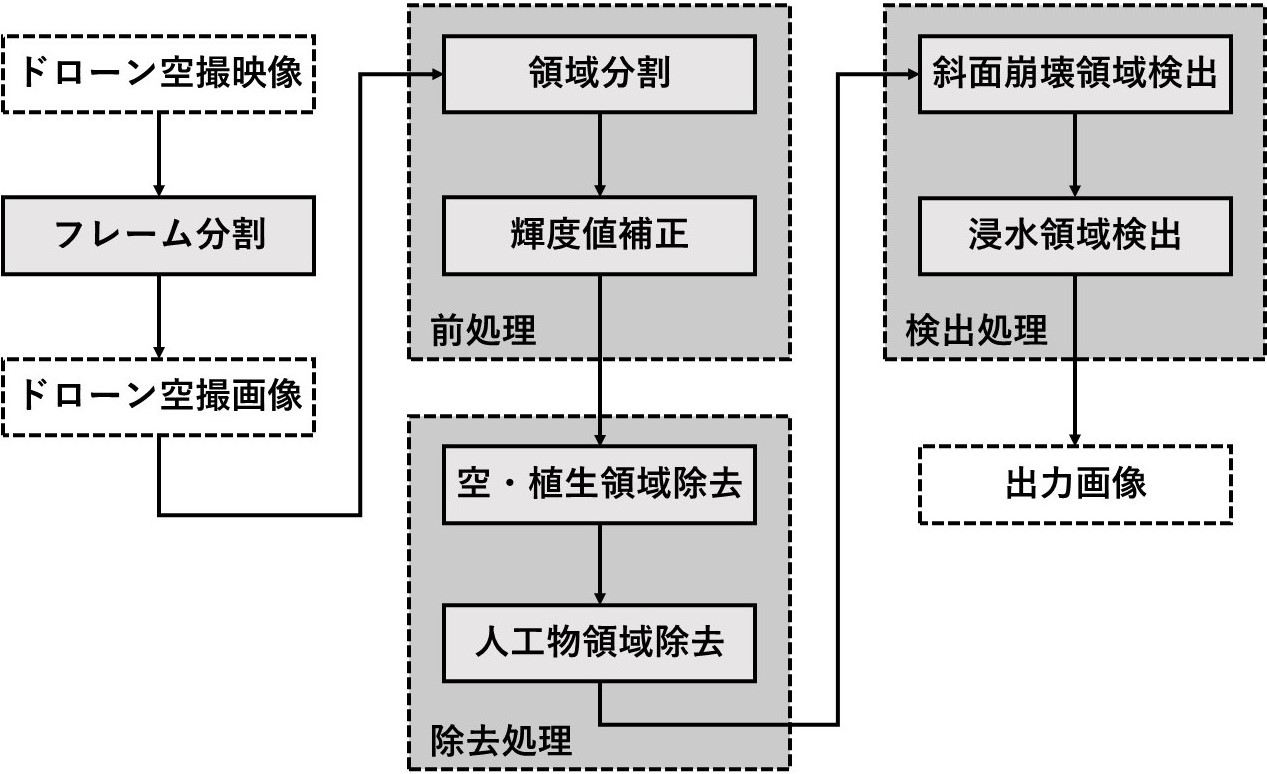
\includegraphics[width=8cm]{img/howto3.jpg}
			% 図のタイトル(キャプション)は下に記述する.
			\caption{提案手法概要図}
			% ラベルの設定
			\label{img01}
		\end{figure}

		\subsection{領域分割}
            本研究では領域ごとに斜面崩壊地と浸水領域を判別するため,まずMean-Shift法による領域分割を行う.Mean-Shift法は近傍の類似した色相を持つ画素郡を同一色に統合し,同一の領域として扱うことができる.

        \subsection{輝度値補正}
            空撮画像は撮影時の天候や時刻によって色相や輝度に偏りが生じるため,CLAHEのアルゴリズム\cite{art05}によって輝度値補正を行う.CLAHEのアルゴリズムは画像を小領域に分割し,小領域毎にヒストグラム平坦化を行う手法で,空撮画像特有の偏りを低減する効果がある.
			
		\subsection{空・植生領域除去}
			ドローンは撮影視点が横方向となることが多く,画像中に空領域を含むことがある.また、山間部では頻繁に画像中に植生領域を含むため,誤検出低減のため空・植生領域を除去する.空領域は青色が強く,輝度値が高いという特徴がある.L*a*b*表色系においてb*値が低いほど青色が強く,L*値が高いほど明るくなる.よって,L*a*b*表色系におけるb*値とL*値にて閾値処理を行い空領域を判別する.また,植生領域は緑色・青色が強いという特徴があるので,空領域と同様に閾値処理を行う.これらの閾値処理結果によりマスク画像を作成し,最終結果から除去する.

		\subsection{人工物領域除去}
			斜面崩壊,浸水,人工物領域は色相が類似していることが多く,2.4節のような色特徴での除去が難しい.そこで,本研究ではテクスチャ特徴量の指標の一つである異質度にて閾値処理を行う.異質度とは画像内の不均一度を示す指標であり,表面が不均一である程高い値を示す.2.4節同様,本処理結果を最終結果から除去する.

		\subsection{斜面崩壊領域検出}
			斜面崩壊領域は赤色が強く,輝度が低いという特徴がある.また,土砂のような不均一な物質を多量に含むため,異質度が高い.これらの特徴を利用し色相,輝度,異質度により閾値処理を行う.

		\subsection{浸水領域検出}
			浸水領域は赤色が強く,輝度が高いという特徴があるため2.6節と同様に閾値処理を行う.そして,これまでの処理を統合したものを最終出力結果とする.


	\section{実験結果}
		本実験では平成29年7月九州北部豪雨のドローン空撮映像\cite{web02}を用いた.\tref{tab01}に空撮映像の詳細を示す.また,\fref{img01}--\fref{img08}に入力画像・現段階での各処理の出力画像を示す.

		\begin{table}[b]
			\centering
			% 表のタイトル(キャプション)は上に記述する
			\caption{使用データ}
			\label{tab01}
			% 表の区切りを設定する
			% c, l, r はそれぞれ「中央寄せ」,「左寄せ」,「右寄せ」を意味する
			% '|' はそれぞれ縦の区切り線を意味する
			\begin{tabular}{l l}
				\hline % \hline は横の区切り線を意味する
				災害名称 & 平成29年7月九州北部豪雨 \\
				撮影箇所 & 福岡県朝倉市赤谷川 \\
				撮影日時 & 平成29年7月7日15時30分 \\
				解像度 & 1920 × 1080 pixel\\
				提供 & 国土地理院 \\ \hline % \\ で改行,\hline で縦を区切る
			\end{tabular}
		\end{table}
		
		% 2つの画像を並べる場合は,minipage 環境を使用する
		\begin{figure}[b]
			\begin{minipage}{0.48\hsize}
				\centering
				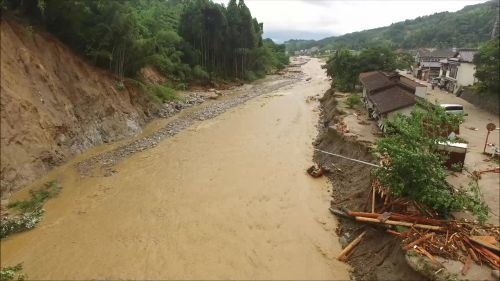
\includegraphics[width=\linewidth]{img/original.jpg}
				\caption{入力画像}
				\label{img01}
			\end{minipage}
			\begin{minipage}{0.48\hsize}
				\centering
				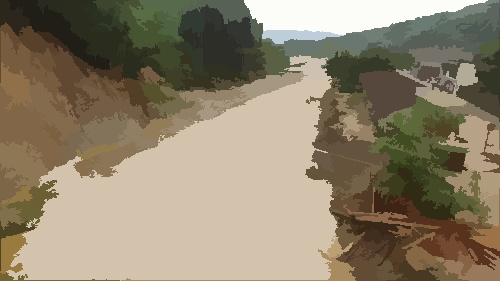
\includegraphics[width=\linewidth]{img/meanshift.jpg}
				\caption{領域分割}
				\label{img02}
			\end{minipage}
		\end{figure}
		\begin{figure}[b]
			\begin{minipage}{0.48\hsize}
				\centering
				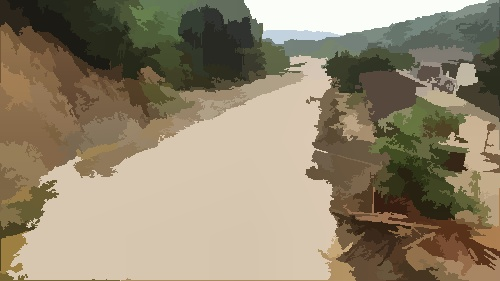
\includegraphics[width=\linewidth]{img/contrast.jpg}
				\caption{輝度値補正}
				\label{img03}
			\end{minipage}
			\begin{minipage}{0.48\hsize}
				\centering
				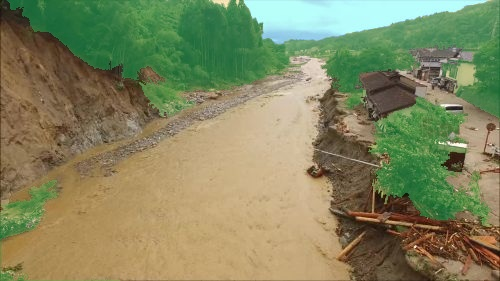
\includegraphics[width=\linewidth]{img/segmentation.jpg}
				\caption{空・植生領域除去(青:空領域,緑:植生領域)}
				\label{img04}
			\end{minipage}
		\end{figure}
		\begin{figure}[t]
			\begin{minipage}{0.48\hsize}
				\centering
				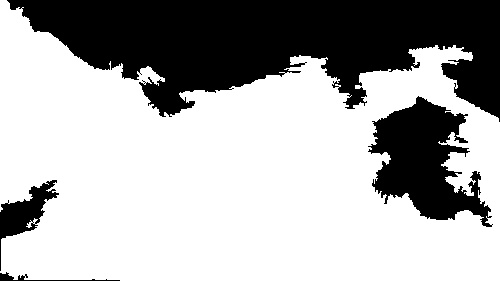
\includegraphics[width=\linewidth]{img/maskNature.jpg}
				\caption{空・植生領域マスク画像}
				\label{img05}
			\end{minipage}
			\begin{minipage}{0.48\hsize}
				\centering
				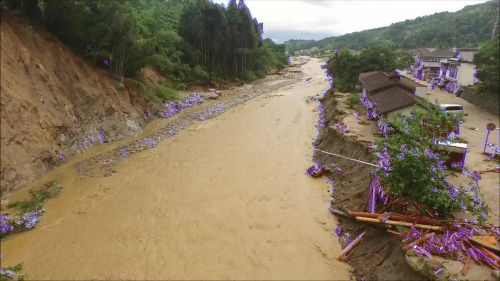
\includegraphics[width=\linewidth]{img/artifact.jpg}
				\caption{人工物領域除去(紫:人工物領域)}
				\label{img06}
			\end{minipage}
		\end{figure}
		\begin{figure}[t]
			\begin{minipage}{0.48\hsize}
				\centering
				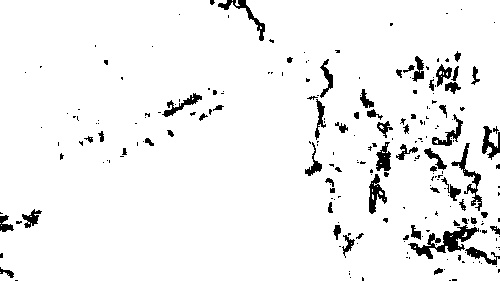
\includegraphics[width=\linewidth]{img/maskArtifact.jpg}
				\caption{人工物領域マスク画像}
				\label{img07}
			\end{minipage}
			\begin{minipage}{0.48\hsize}
				\centering
				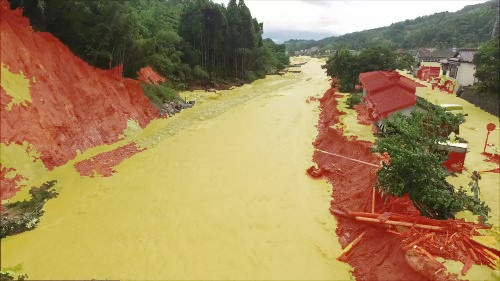
\includegraphics[width=\linewidth]{img/result.jpg}
				\caption{出力画像(赤:斜面崩壊領域,黃:浸水領域)}
				\label{img08}
			\end{minipage}
		\end{figure}

	
	\section{まとめ・今後の予定}
		本実験ではドローン空撮映像から斜面崩壊・浸水領域を検出する手法を提案した.現状の問題点として人工物領域除去の精度が低いことや,斜面崩壊・浸水領域同士の誤検出,検出精度の定量的な評価が未実装である点が挙げられる.また,浸水領域に関し,既存の河川と災害によって水没した浸水箇所の判別は未実装である.\\
		 今後はこれらの誤検出改善・実装を進め,システムの精度向上を目指す.

	\section{参考文献}
		
		% 参考文献はbibtexを用いて作成する。文献を参照するには\cite{鈴木:論文06}、\cite{Web01}とする。

% 参考文献の表示
\bibliographystyle{junsrt}   % 参考文献の並び順を指定
\bibliography{bib/myref.bib} % \bibliography{参考文献ファイルへのパス}

\end{document}
